\chapter{Algorithm}

This chapter presents all the passes which are applied to the code of the method until the final result is achieved.
Each pass is represented by a visitor which usually first collects information about the change that has to be made and
then alters the code.

\section{Renaming local variables to unique names}

This code transformation is needed in order to avoid name clashes later on, when the static nested class which
holds the variables potentially used after returning from a recursive call (both formal parameters and local variables)
is generated. The fields of this class will simulate the stack frame of the method.

The JVMS (Java Virtual Machine Specification)\abbrev{JVMS}{Java Virtual Machine Specification} states the
following\footnote{\url{http://docs.oracle.com/javase/specs/jvms/se8/html/jvms-2.html#jvms-2.6.1}}:

\begin{quote}
    The Java Virtual Machine uses local variables to pass parameters on method invocation. On class method invocation,
    any parameters are passed in consecutive local variables starting from local variable 0. On instance method invocation,
    local variable 0 is always used to pass a reference to the object on which the instance method is being invoked
    (\code{this} in the Java programming language). Any parameters are subsequently passed in consecutive local
    variables starting from local variable 1.
\end{quote}

In the context of this refactoring, the recursive call is defined only as a method call expression whose qualifier is
either absent or \code{this}, so the target reference of the instance method invocation never changes. This is why it is
not a field of the frame class. In the case of class method invocations, there is no target reference (\code{this}).

JLS specifies that\footnote{\url{https://docs.oracle.com/javase/specs/jls/se8/html/jls-6.html#jls-6.4}}:
\begin{quote}
    It is a compile-time error if the name of a formal parameter is used to declare a new variable within the body of
    the method, constructor, or lambda expression, unless the new variable is declared within a class declaration
    contained by the method, constructor, or lambda expression.

    It is a compile-time error if the name of a local variable v is used to declare a new variable within the scope of
    v, unless the new variable is declared within a class whose declaration is within the scope of v.
\end{quote}

This means that all the names of formal parameters and local variables whose scopes overlap are unique in the method
body. In other words, a compile-time error occurs for the program in
\labelindexref{Figure}{img:attempted-shadowing-of-a-local-variable}, but not for the program in
\labelindexref{Figure}{img:no-shadow}.

\fig[width=4in]{src/img/attempted-shadowing-of-a-local-variable.png}{img:attempted-shadowing-of-a-local-variable}{Attempted shadowing of a local variable}
\fig[width=4in]{src/img/no-shadow.png}{img:no-shadow}{Two non-overlapping scopes}

In the second example, it also means that the storage for the first \code{i} variable can be reused as the storage for
the second \code{i} variable, thus reducing the number of fields in the generated frame class, as at any moment during
the execution of the method, only one variable (formal parameter or local variable) of a certain name is in scope,
meaning that its value can be used in the code.

There are still problems if there is another variable in the method which shares the same name with other variable, but
whose type is different. If this other variable is not renamed, when generating the frame class, a compile-time error
will occur because JLS specifies that\footnote{\url{https://docs.oracle.com/javase/specs/jls/se8/html/jls-8.html#jls-FieldDeclaration}}:
\begin{quote}
    It is a compile-time error for the body of a class declaration to declare two fields with the same name.
\end{quote}

So all the relevant variables in the method (formal parameters and local variables) will be collected as fields of a
static nested frame class, which will be used by the recursive method to save the state of the method call when
recursing, thus simulating the call stack. The rule is that for all the variables with the same name and type, there
will be only one corresponding field in the frame class, but if there are variables with the same name, but different
type, each variable in a type group will have a different name and a different corresponding frame class field.

In other words, the first pass ensures that all the variables in a method which have the same name also have the same
type.

TODO: Add example of renaming.

\section{Replacing \code{foreach} loops with \code{for} loops}

In Java, the \code{for} statement\footnote{\url{https://docs.oracle.com/javase/specs/jls/se8/html/jls-14.html#jls-14.14}}
has two forms: the basic one and the enhanced one. Since the meaning of the enhanced \code{for} statement is given by
translation into a basic \code{for} statement\footnote{\url{https://docs.oracle.com/javase/specs/jls/se8/html/jls-14.html#jls-14.14.2}},
the enhanced form is merely syntactic sugar for the basic one.

This pass first collects all the enhanced \code{for} statements in the method body which contain at least one recursive
call in pre-order fashion by using a visitor processing children nodes before the current node. Then it replaces these
statements by their equivalent basic \code{for} statements. This conversion is necessary because control flow needs to
be explicit for later stages in the refactoring process. The \textit{Condition} and \textit{Update} part of a \code{for}
statement in particular need to be explicit because they get executed after returning from a recursive call in the body
of the \code{for} statement.

There are two cases for this conversion: the first when the type of \textit{Expression} is a subtype of
\texttt{Iterable} (exemplified in \labelindexref{Figure}{img:foreach-to-iterator-for-before} and
\labelindexref{Figure}{img:foreach-to-iterator-for-after}) and the second when \textit{Expression} has an array type
\texttt{T[]} (exemplified in \labelindexref{Figure}{img:foreach-to-indexed-for-before} and
\labelindexref{Figure}{img:foreach-to-indexed-for-after}), where \textit{Expression} is the value over which the
enhanced \code{for} statement iterates.

\fig[height=0.5in]{src/img/foreach-to-iterator-for-before.png}{img:foreach-to-iterator-for-before}{\code{Foreach} loop to iterator \code{for} loop conversion (before)}
\fig[height=0.625in]{src/img/foreach-to-iterator-for-after.png}{img:foreach-to-iterator-for-after}{\code{Foreach} loop to iterator \code{for} loop conversion (after)}
%\fig[width=.3\textwidth]{src/img/foreach-to-indexed-for-before.png}{img:foreach-to-indexed-for-before}{\code{Foreach} loop to indexed \code{for} loop conversion (before)}
%\fig[width=.4\textwidth]{src/img/foreach-to-indexed-for-after.png}{img:foreach-to-indexed-for-after}{\code{Foreach} loop to indexed \code{for} loop conversion (before)}
\begin{figure}[!tbp]
    \centering
    \begin{minipage}[b]{0.45\textwidth}
        \begin{center}
            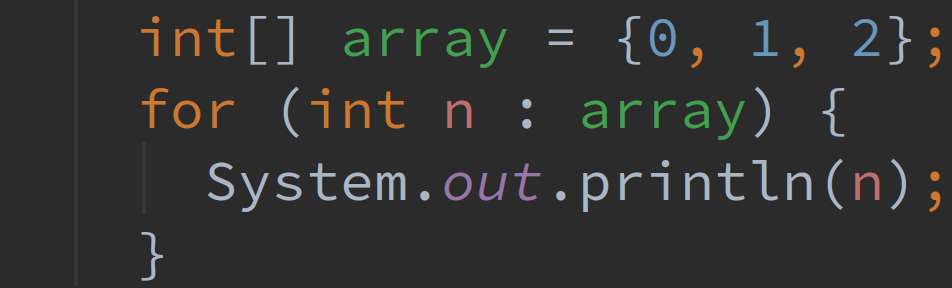
\includegraphics[height=0.5in]{src/img/foreach-to-indexed-for-before.png}
            \caption{\code{Foreach} loop to indexed \code{for} loop conversion (before) \label{img:foreach-to-indexed-for-before}}
        \end{center}
    \end{minipage}
    \hfill
    \begin{minipage}[b]{0.45\textwidth}
        \begin{center}
            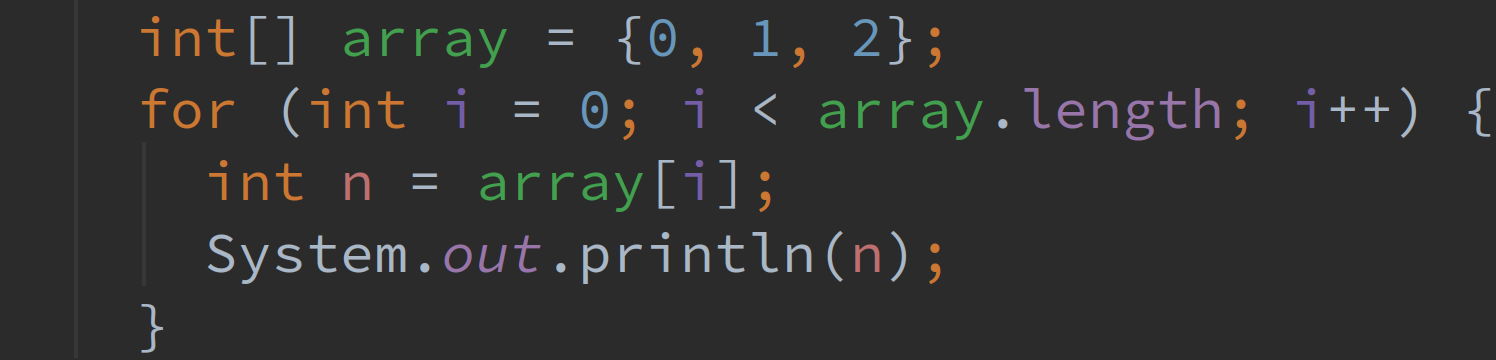
\includegraphics[height=0.625in]{src/img/foreach-to-indexed-for-after.png}
            \caption{\code{Foreach} loop to indexed \code{for} loop conversion (before) \label{img:foreach-to-indexed-for-after}}
        \end{center}
    \end{minipage}
\end{figure}
%These two conversions are carried out using the ones that Intellij IDEA provides as intentions.